\documentclass[12pt,a4paper]{article}
\usepackage[utf8]{inputenc}
\usepackage[OT1]{fontenc}
\usepackage{amsmath}
\usepackage{amsfonts}
\usepackage{amssymb}
\usepackage{graphicx}
\usepackage{tikz}
\usepackage{pgfplotstable}
\usepackage{mathtext}

\usepackage[T1]{fontenc}
\usepackage[utf8]{inputenc}
\usepackage[english, bulgarian, russian]{babel}

\usepackage{tikz}
\usepackage{pgfplots}
\usepackage{indentfirst}
\usepackage[export]{adjustbox}
\usepackage{multirow}
\usepackage{geometry} \geometry{verbose,a4paper,tmargin=2cm,bmargin=2cm,lmargin=1.5cm,rmargin=1.5cm}

\graphicspath{{Images/}}
\usepackage[left=2cm,right=2cm,top=2cm,bottom=2cm]{geometry}
\usepackage{wrapfig}
\usepackage{setspace}
\usepackage{indentfirst}
\usepackage{subfigure}


\begin{document}

\begin{titlepage}
  \begin{center}
    \huge
    Московский Физико-технический Институт
    
    (Национальный исследовательский университет)
    \vspace{0.5cm}

   
    \vspace{0.25cm}
 
    \vfill
 
    \vfill

    \textsc{\bf{Отчет о выполнении работы 2.1.6}}\\[3mm]
    
    {\LARGE  Эффект Джоуля-Томсона}
  \bigskip
    \vfill
    
\end{center}
\vfill
\begin{flushright}

    Выполнили студентки 1 курса
    
    ФБМФ, группа Б06-103

    Попеску Полина
    
    
    Фитэль Алёна

\end{flushright}
\bigskip


\vfill

\begin{center}
  Долгопрудный, 2022 г.
\end{center}
\end{titlepage}

\section{Введение}

\textbf{Цель работы:} 1) определение изменения температуры углекислого газа при протекании через малопроницаемую перегородку при разных начальных значениях давления и температуры; 2) вычисление по результатам опытов коэффициентов Ван-дер-Ваальса $"a"$ и $"b"$.

\textbf{В работе используются:} трубка с пористой перегородкой; труба Дьюара; термостат; термометры; дифференциальная термопара; микровольтметр; балластный баллон; манометр.

\section{Теоретический материал}

Эффектом Джоуля–Томсона называется изменение температуры газа, медленно протекающего из области высокого в область низкого давления в условиях хорошей тепловой изоляции. 
В разреженных газах, которые приближаются по своим свойствам к идеальному газу, при таком течении температура газа не меняется. 
Эффект Джоуля–Томсона демонстрирует отличие исследуемого газа от идеального.

Рассмотрим стационарный поток газа между произвольными сечениями I и II трубки (до перегородки и после неё).
Пусть, для определённости, через трубку прошёл 1 моль углекислого газа; $\mu$ — его молярная масса. 
Молярные объёмы газа, его давления и отнесённые к молю внутренние энергии газа в сечениях I и II обозначим соответственно $V_1,\ P_1,\ U_1\ и\ V_2,\ P_2,\ U_2$. 
Для того чтобы ввести в трубку объём $V_1$, над газом нужно совершить работу $A_1 = P_1V_1$. 
Проходя через сечение II, газ сам совершает работу $A_2 = P_2V_2$. 
Так как через боковые стенки не происходит ни обмена теплом, ни передачи механической энергии, то
\begin{equation}
    A_1 - A_2 = \left( U_2 + \frac{\mu v_2 ^2}{2}\right) - \left(U_1 + \frac{\mu v_1^2}{2}\right)
\end{equation}

В уравнении (1) учтено изменение как внутренней (первые члены в скобках), так и кинетической (вторые члены в скобках) энергии газа. 
Подставляя в (1) написанные выражения для $A_1$ и $A_2$ и перегруппировывая члены, найдём
\begin{equation}
    H_1 - H_2 = (U_1 + P_1 V_1) - (U_2 + P_2 V_2) = \frac 1 2\mu (v_2^2 - v_1^2).
\end{equation}
Сделаем несколько замечаний. 
Прежде всего отметим, что в процессе Джоуля–Томсона газ испытывает в пористой перегородке существенное трение, приводящее к её нагреву. 
Потери энергии на нагрев трубки в начале процесса могут быть очень существенными и сильно искажают ход явления. 
После того как температура трубки установится и газ станет уносить с собой все выделенное им в пробке тепло, формула (1) становится точной, если, конечно, теплоизоляция трубки достаточно хороша и не происходит утечек тепла наружу через её стенки.

Второе замечание связано с правой частью (2). 
Процесс Джоуля–Томсона в чистом виде осуществляется лишь в том случае, если правой частью можно пренебречь, т. е. если макроскопическая скорость газа с обеих сторон трубки достаточно мала. 
У нас сейчас нет критерия, который позволил бы установить, когда это можно сделать. 
Поэтому мы отложим на некоторое время обсуждение вопроса о правой части (2), а пока будем считать, что энтальпия газа не меняется в соответствии с формулой.
В соответствии с этим получаем
\begin{equation}
    \mu_{д-т} = \frac {\Delta T}{\Delta P} \approx \frac {\frac {2a}{RT} - b}{C_p}
\end{equation}

Из формулы (3) видно, что эффект Джоуля–Томсона для не очень плотного газа зависит от соотношения величин a и b, которые оказывают противоположное влияние на знак эффекта. 
Если силы взаимодействия между молекулами велики, так что превалирует «поправка на давление», то основную роль играет член, содержащий $a$, и $$\frac {\Delta T} {\Delta P} > 0$$
т. е. газ при расширении охлаждается ($\Delta T < 0$, т. к. всегда $\Delta P < 0$).

В обратном случае (малые $a$) $$\frac {\Delta T} {\Delta P} < 0$$ т. е. газ нагревается. 
Как следует из формулы (3), при темепературе $T_i = \frac{2a}{Rb}$ коэффициент $\mu_{д-т}$ обращается в нуль.
Тогда по формулам связи параметров газа Ван-дер-Ваальса с критическими параметрами получаем:
\begin{equation}
    T_{инв} = \frac{27}4 T_{кр}
\end{equation} 

При температуре $T_{инв}$ эффект Джоуля–Томсона меняет знак: ниже температуры инверсии эффект положителен ($\mu_{д-т}$ > 0, газ охлаждается), выше $T_{инв}$ эффект отрицателен ($\mu_{д-т}$ < 0, газ нагревается).

Вернёмся к влиянию правой части уравнения (2) на изменение температуры расширяющегося газа. 
Для этого сравним изменение температуры, происходящее вследствие эффекта Джоуля–Томсона, с изменением температуры, возникающим из-за изменения кинетической энергии газа. 
Увеличение кинетической энергии газа вызывает заметное и приблизительно одинаковое понижение его температуры как у реальных, так и у идеальных газов. 
Поэтому при оценках нет смысла пользоваться сложными формулами для газа Ван-дер-Ваальса.

Заменяя в формуле (2) $U$ через $C_V T$ и $P V$ через $R T$, найдём
\begin{equation*}
    (R + C_V)(T_1 - T_2) = \mu \frac{v_2^2 - v_1^2}2
\end{equation*}
или 
\begin{equation*}
    \Delta T = \frac{\mu}{2C_p} (v_2^2-v_1^2).
\end{equation*}

В условиях нашего опыта расход газа $Q$ на выходе из пористой перегородки не превышает $10\ см^3/с$, а диаметр трубки равен $3\ мм$. Поэтому
\begin{equation*}
    v_2 \le \frac{4Q}{\pi d^2} = \frac{4\cdot 10\ см^3/c}{3.14 \cdot (0.9)^2\ см^2} \approx 140\ см/c.
\end{equation*}

Скорость $v_1$ газа у входа в пробку относится к скорости $v_2$ у выхода из неё как давление $P_2$ относится к давлению $P_1$. 
В нашей установке $P_1 = 4$ атм, a $P_2 = 1$ атм, поэтому

\begin{equation*}
    v_1 = \frac {P_2}{P_1}v_2 = \frac{1\ атм}{4\ атм} \cdot 140\ см/с=35\ см/с.
\end{equation*}

Для углекислого газа имеем $\mu = 44\ г/моль,\ C_p = 40 \frac{Дж}{моль\cdot K} \Rightarrow \Delta T = 7\cdot 10^{-4} K$
Это изменение температуры ничтожно мало по сравнению с измеряемым эффектом (несколько градусов).

В данной лабораторной работе исследуется коэффициент дифференциального эффекта Джоуля–Томсона для углекислого газа. 
По экспериментальным результатам оценивается коэффициент теплового расширения, постоянные в уравнении Ван-дер-Ваальса и температура инверсии углекислого газа. 
Начальная температура газа $T_1$ задаётся термостатом. 
Измерения проводятся при трёх температурах: комнатной, $30^oC$ и $40^oC$.

\subsection*{Экспериментальная установка}
\begin{figure}[htp]
    \centering
    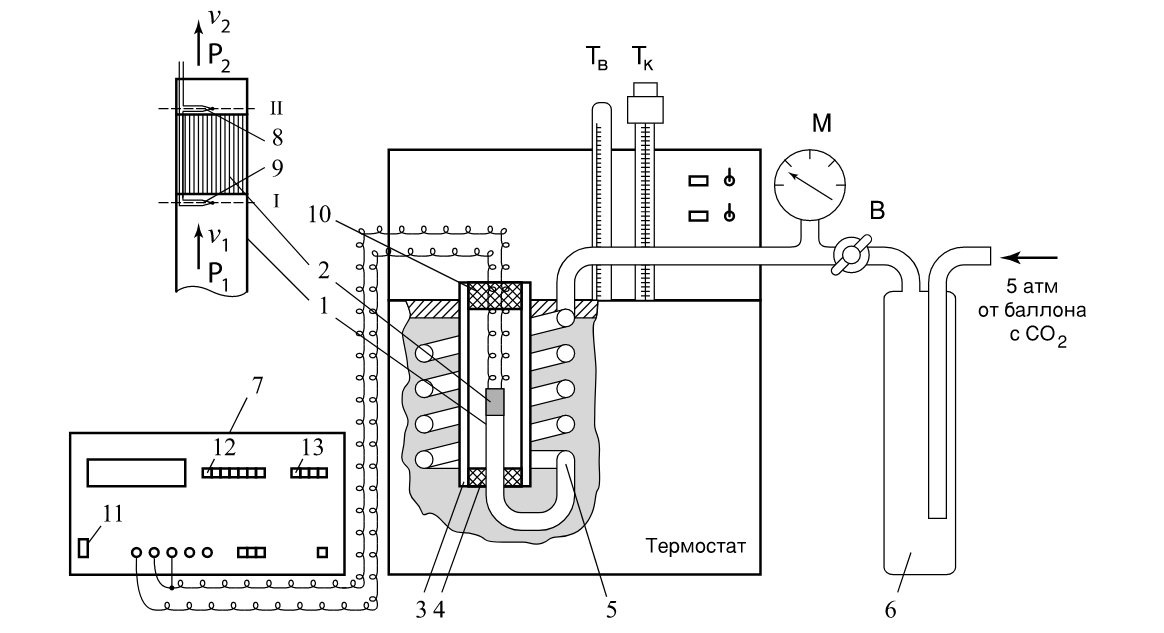
\includegraphics[width=0.7\linewidth]{scheme.png}
    \caption{Схема установки}
\end{figure}
Схема установки для исследования эффекта Джоуля–Томсона в углекислом газе представлена на рисунке 1. 
Основным элементом установки является трубка 1 с пористой перегородкой 2, через которую пропускается исследуемый газ. 
Трубка имеет длину 80 мм и сделана из нержавеющей стали, обладающей, как известно, малой теплопроводностью. 
Диаметр трубки $d$ = 3 мм, толщина стенок 0,2 мм. Пористая перегородка расположена в конце трубки и представляет собой стеклянную пористую пробку со множеством узких и длинных каналов. 
Пористость и толщина пробки ($l$ = 5 мм) подобраны так, чтобы обеспечить оптимальный поток газа при перепаде давлений $\Delta P \le$ 4 атм (расход газа составляет около $10\ см^3/с$); 
при этом в результате эффекта Джоуля–Томсона создаётся достаточная разность температур.

Углекислый газ под повышенным давлением поступает в трубку через змеевик 5 из балластного баллона 6. 
Медный змеевик омывается водой и нагревает медленно протекающий через него газ до температуры воды в термостате. 
Температура воды измеряется термометром $T_в$, помещённым в термостате. 
Требуемая температура воды устанавливается и поддерживается во время эксперимента при помощи контактного термометра $T_к$.

Давление газа в трубке измеряется манометром М и регулируется вентилем В (при открывании вентиля В, т. е. при повороте ручки против часовой стрелки, давление $P_1$ повышается). 
Манометр М измеряет разность между давлением внутри трубки и наружным (атмосферным) давлением. Так как углекислый газ после пористой перегородки выходит в область с атмосферным давлением $P_2$, то этот манометр непосредственно измеряет перепад давления на входе и на выходе трубки $\Delta P = P_1 - P_2$.

Разность температур газа до перегородки и после неё измеряется дифференциальной термопарой медь — константан. 
Константановая проволока диаметром 0,1 мм соединяет спаи 8 и 9, а медные проволоки (того же диаметра) подсоединены к цифровому вольтметру 7. 
Отвод тепла через проволоку столь малого сечения пренебрежимо мал. 
Для уменьшения теплоотвода трубка с пористой перегородкой помещена в трубу Дьюара 3, стенки которой посеребрены, для уменьшения теплоотдачи, связанной с излучением. 
Для уменьшения теплоотдачи за счёт конвекции один конец трубы Дьюара уплотнен кольцом 4, а другой закрыт пробкой 10 из пенопласта. 
Такая пробка практически не создаёт перепада давлений между внутренней полостью трубы и атмосферой.

 
\section{Обработка результатов измерений}
\subsection{Определение коэффициента Джоуля-Томсона}

Проведём измерение зависимости $ \Delta T $ от $ \Delta P $ для разных значений температур, по которым проведём аппроксимацию зависимости $ \Delta T $ от $ \Delta P $, чтобы определить коэффициент Джоуля-Томсона. На рисунке \ref{ris} изображены графики зависимостей. Вычислим $ \mu_\text{Д--Т} = \frac{dT}{dP} $, используя метод наименьших квадратов.

 \begin{figure}[h!]
    \centering
    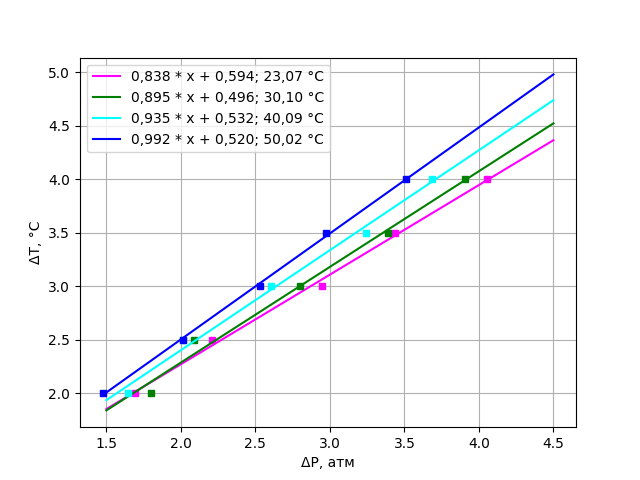
\includegraphics[scale=0.8]{plot.png}
	\caption{Графики зависимости $ \Delta T $ от $ \Delta P $}
	\label{ris}
\end{figure}

Результаты вычислений заносим в таблицу \ref{tab:my-table}.
\label{koef}
\begin{table}[h]
	\centering
	\begin{tabular}{|c|c|c|c|}
		\hline
		$ T $, $ ^\circ C $ & $ \mu_\text{Д--Т} $, К/атм & $ \sigma_{\mu_\text{Д--Т}} $, К/атм \\ \hline
		23,07 & 0,84 & 0,02 \\ \hline
		30,10 & 0,90 & 0,04 \\ \hline
		40,09 & 0,94 & 0,04 \\ \hline
		50,02 & 0,99 & 0,01 \\ \hline
		
	\end{tabular}
	\caption{Результаты измерений $ \mu_\text{Д--Т} $}
	\label{tab:my-table}
\end{table}

\subsection{Вычисление параметров газа Ван-дер-Ваальса}

Вычислим параметры газа Ван-дер-Ваальса, используя коэффициенты $ \mu_\text{Д--Т} $, полученные в \ref{koef}, для разных пар температур.

Пользуясь формулой (3), получим 

\[ \left\{ \begin{aligned}
	 a &= \frac{\left(\mu_1 - \mu_2\right)C_PRT_1T_2}{2\left(T_2-T_1\right)}, \\
	b &= \frac{C_P(\mu_2T_2-\mu_1T_1)}{T_1-T_2}. \end{aligned} \right. \]

Для различных комбинаций температур  вычисляем параметры $a$ и $b$ газа Ван-дер-Ваальса. Результаты вычислений заносим в таблицы 2 и 3, в которых соответственно стоят  параметры $a$ и $b$ в единицах измерения $\displaystyle \frac{\text{Па}\cdot\text{м}^6}{\text{моль}^2} $  и $10^{-6}$$\displaystyle\text{ }\frac{\text{м}^3}{\text{моль}}$. 


\begin{table}[h!]
\centering
\begin{tabular}{|c|c|c|c|c|}
\hline
\textbf{T, °C} & \textbf{23,07} & \textbf{30,10} & \textbf{40,09} & \textbf{50,02} \\ \hline
\textbf{23,07} & -              & 0,89$\pm$0,05     & 0,63$\pm$0,04     & 0,66$\pm$0,04     \\ \hline
\textbf{30,10} & -              & -              & 0,45$\pm$0,02     & 0,59$\pm$0,02     \\ \hline
\textbf{40,09} & -              & -              & -              & 0,70$\pm$0,04     \\ \hline
\textbf{50,02} & -              & -              & -              & -              \\ \hline
\end{tabular}
	\caption{Результаты измерения $a$ газа Ван-дер-Ваальса}
\end{table}

\begin{table}[h!]
\centering
\begin{tabular}{|c|c|c|c|c|}
\hline
\textbf{T, °C} & \textbf{23,07} & \textbf{30,10} & \textbf{40,09} & \textbf{50,02} \\ \hline
\textbf{23,07} & -              & 96$\pm$8          & 76$\pm$6          & 78$\pm$6          \\ \hline
\textbf{30,10} & -              & -              & 62$\pm$5          & 72$\pm$6          \\ \hline
\textbf{40,09} & -              & -              & -              & 81$\pm$7          \\ \hline
\textbf{50,02} & -              & -              & -              & -              \\ \hline
\end{tabular}
	\caption{Результаты измерения $b$ газа Ван-дер-Ваальса}

\end{table}

Таким образом,
\begin{equation*}
    a = 0,65 \pm 0,09 \frac{\text{Па}\cdot\text{м}^6}{\text{моль}^2}
\end{equation*}

\begin{equation*}
    b = (0,78 \pm 0,15) \cdot 10^{-4} \text{ }\frac{\text{м}^3}{\text{моль}}
\end{equation*}

Согласно справочнику для углекислого газа \[ a = 0,36 \text{ } \frac{\text{Па}\cdot\text{м}^6}{\text{моль}^2}, \] \[ b = 0,42\cdot 10^{-4} \text{ }\frac{\text{м}^3}{\text{моль}}. \]

\subsection{Уравнение Бертло}


Рассмотрим другое приближение идеального газа: по Бертло.
\[\left( p + \dfrac{a}{TV^2} \right) (V - b) = RT\]
\[pV + \dfrac{a}{TV} - \dfrac{ab}{TV^2} - bp = RT\]
\[\left(\dfrac{\partial V}{\partial T} \right)_p \left( p - \dfrac{a}{TV^2} + \dfrac{2ab}{TV^3} \right) - \dfrac{a}{VT^2} + \dfrac{ab}{T^2 V^2} = R\]
\[\left(\dfrac{\partial V}{\partial T} \right)_p = \dfrac{(RV^2T^2 + aV - ab)(V-b)}{T \left( RT^2V^2 - 2a(V-b) + \dfrac{2ab(V-b)}{V} \right)} \Rightarrow \mu = \dfrac{\dfrac{3a}{RT^2} - b}{C_p} \]
Для него получаем:

\begin{equation*} 
 		\begin{cases}
   			\mu_1 = \dfrac{\dfrac{3a}{RT_1^2} - b}{3,5R}\\
   			\\
   			\mu_2 = \dfrac{\dfrac{3a}{RT_2^2} - b}{3,5R}\\
   			\\
   			\end{cases}
	\end{equation*}
	из этой системы получаем, что 
	\[a = \dfrac{7R^2(\mu_2 - \mu_1)}{6 \left( \dfrac{1}{T_1^2} - \dfrac{1}{T_2^2} \right)} \]
	\[b = \dfrac{3a}{RT_1^2} - 3,5R \mu_1 \]
Для различных комбинаций температур  вычисляем параметры $a$ и $b$ газа Ван-дер-Ваальса. Результаты вычислений заносим в таблицы 2 и 3, в которых соответственно стоят  параметры $a$ и $b$ в единицах измерения $\displaystyle \frac{\text{Па}\cdot\text{м}^6}{\text{моль}^2} $  и $10^{-6}$$\displaystyle\text{ }\frac{\text{м}^3}{\text{моль}}$. 


\begin{table}[h!]
\centering
\begin{tabular}{|c|c|c|c|c|}
\hline
\textbf{T, °C} & \textbf{23,07} & \textbf{30,10} & \textbf{40,09} & \textbf{50,02} \\ \hline
\textbf{23,07} & -              & 0,89$\pm$0,05     & 0,65$\pm$0,04     & 0,68$\pm$0,04     \\ \hline
\textbf{30,10} & -              & -              & 0,46$\pm$0,02     & 0,60$\pm$0,02     \\ \hline
\textbf{40,09} & -              & -              & -              & 0,74$\pm$0,04     \\ \hline
\textbf{50,02} & -              & -              & -              & -              \\ \hline
\end{tabular}
	\caption{Результаты измерения $a$ газа Ван-дер-Ваальса}
\end{table}

\begin{table}[h!]
\centering
\begin{tabular}{|c|c|c|c|c|}
\hline
\textbf{T, °C} & \textbf{23,07} & \textbf{30,10} & \textbf{40,09} & \textbf{50,02} \\ \hline
\textbf{23,07} & -              & 24,4$\pm$ 0,06         & 24,4$\pm$0,04          & 24,4$\pm$0,03          \\ \hline
\textbf{30,10} & -              & -              & 26,0$\pm$0,1          & 26,0$\pm$0,4          \\ \hline
\textbf{40,09} & -              & -              & -              & 27,2$\pm$0,6          \\ \hline
\textbf{50,02} & -              & -              & -              & -              \\ \hline
\end{tabular}
	\caption{Результаты измерения $b$ газа Ван-дер-Ваальса}

\end{table}

Таким образом,
\begin{equation*}
    a = 0,67 \pm 0,09 \frac{\text{Па}\cdot\text{м}^6}{\text{моль}^2}
\end{equation*}

\begin{equation*}
    b = (25,4 \pm 0,09) \cdot 10^{-6} \text{ }\frac{\text{м}^3}{\text{моль}}
\end{equation*}

\subsection{Вычисление температуры инверсии}

Используя формулу (4), по полученным параметрам газа Ван-дер-Ваальса вычислим $ T_\text{инв} $. Результаты вычислений занесём в таблицу \ref{tab:temp}.


\begin{table}[h!]
\centering
\begin{tabular}{|c|c|c|c|c|}
\hline
\textbf{T, °C} & \textbf{23,07} & \textbf{30,10} & \textbf{40,09} & \textbf{50,02} \\ \hline
\textbf{23,07} & -              & 2214$\pm$220       & 2014$\pm$200       & 2036$\pm$200       \\ \hline
\textbf{30,10} & -              & -              & 1761$\pm$160       & 1992$\pm$180       \\ \hline
\textbf{40,09} & -              & -              & -              & 2081$\pm$220       \\ \hline
\textbf{50,02} & -              & -              & -              & -              \\ \hline
\end{tabular}
\caption{Результаты вычисления температуры инверсии}
	\label{tab:temp}
\end{table}

Таким образом,
\begin{equation*}
    T_\text{инв} = 2020 \pm 480 К
\end{equation*}

Для углекислого газа, согласно справочнику  \[ T_\text{инв} = 2053 \text{ K}.\]

\section{Вывод}
В ходе работы мы проверили наличие эффекта Джоуля-Томсона для углекислого газа, что доказывает его отличие от модели идеального газа, а также расчитали параметры данного газа для модели газа Ван-дер-Ваальса и модели Бертло. 
Погрешности измерений в основном связаны с погрешностями определения $ \mu_{д-т} = \frac {\Delta T}{\Delta P}$,которые обоснованы неадиабатичностью установки, что на самом деле говорит о том, что энтальпия в рассматриваемом процессе не сохраняется, вследствие чего трудно говорить о процессе Джоуля-Томсона в данной установке. В пределах погрешностей полученные значения параметра $a$ газа по уравнению Ван-дер-Ваальса и по уравнению Бертло совпадают, но  $b$ - нет. Уравнение Бертло учитывает, в отлисие от классического уравнения Ван-дер-Ваальса то, что газокинетический параметр $a$ зависит от температуры $T$. 
Несоответствие полученных значений для обоих моделей газа с табличными связано с тем, что уравнение газа Ван-дер-Ваальса, как и его уравнение с поправкой на один из коэффициентов - уравнение Бертло-  используются лишь для качественного описания процессов, происходящих с реальными газами и количественный подход к этим уравнениям дает результаты не соответствующие опыту. 



\end{document}
